\chapter{Darba praktiskā daļa}

\section{\textit{Git}}
Darba izstrādē versiju vadība bija ļoti svarīga. Izstrādes gaitā izdevās atklāt un izlabot vairākas kļūdas, izmantojot \textit{Git} VCS un \textit{GitHub} sniegtās iespējas. Noderīgas ir trešo pušu rīku integrācijas ar GitHub. Darbā izmantotas divas, kas nedaudz apskatītas \ref{Testing} nodaļā. Galu galā tika izveidoti trīs repozitoriji, kuri atrodas uz GitHub:
\begin{describe}
	\item Mājaslapas izstrādei -- https://github.com/RihardsT/access_page
	\item Servera konfigurēšanai -- https://github.com/RihardsT/access_page_cookbook
	\item Teorētiskajam aprakstam -- https://github.com/RihardsT/thesis
\end{describe}

\textit{Git} repozitorija uzstādīšana ir ļoti vienkārša. Jebkurā eksistējošā direktorijā ir iespējams uzstādīt versiju vadību. Lai uzstādītu GitHub, kā attālinātu repozitorija serveri, to nepieciešams arī norādīt Git. Servera konfigurācijas repozitorijs tik izveidots no jau eksistējošā direktorijā, tāpēc bija jāveic šādas komandas:
\begin{lstlisting}
	git init
	git remote add origin  https://github.com/RihardsT/access_page_cookbook
	git push -u origin master
	git checkout -b develop
\end{lstlisting}
Komandas \textit{git push} karogs "\texttt{-u}" jeb "\texttt{--set-upstream}" uzstāda attālināto repozitorija adresi, kas turpmāk tiks lietota pēc noklusējuma veicot \textit{git push} komandu. Izveidojot repozitoriju, \textit{Git} pēc noklusējuma izveido tikai pamatzaru - \textit{master}. Pieņemts, ka uz pamatzara aktīva izstrāde netiek veikta, tajā izmaiņas tiek tikai iepludinātas. Tāpēc tika izveidots izstrādes zars - \textit{develop}, veicot \textit{checkout} komandu, kuru izmanto, lai nomainītu zaru uz kura atrodas. Komandas "-b" karogs norāda, ka jāizveido jauns zars uz to jāpārslēdzas.

Mājaslapas repozitorijam tika pielāgota \textit{Gitflow} darbplūsma, kas aprakstīta \ref{Branching} nodaļā. Praktiski \textit{Gitflow} darbplūsma nosaka tikai izmantojamos zaru nosaukumus un nosaka kā jāveic zarošanās konkrētos gadījumos, piemēram, pievienojot jaunu funkcionalitāti vai veicot kļūdu labojumus. Tādejādi \textit{Gitflow} darbplūsmai ir iespējams sekot ievērojot tās noteiktajām konvencijām. Lai atvieglotu darbu ar \textit{Gitflow} tika uzstādīts \textit{Git} paplašinājums darbam ar \textit{Gitflow} \url{https://github.com/petervanderdoes/gitflow-avh}. Uzstādot šo paplašinājumu, jaunu vai eksistējošu repozitoriju ir iespējams inicializēt kā \textit{Gitflow} repozitoriju:
\begin{lstlisting}
	git flow init --defaults
\end{lstlisting}
Karogs "\texttt{--defaults}" norāda, ka tiks izmantoti noklusējuma zaru nosaukumi: \textit{feature release hotfix support}. Izmantojot šo \textit{Git} paplašinājumu, tiek nodrošināta atbilstība \textit{Gitflow} darbplūsmai. Piemēram, sākot ieviest jaunu funkcionalitāti, jaunais zars tiks izveidots no izstrādes zara un to beidzot, tas tajā tiks iepludināts. Veicot kļūdu labojumus, paplašinājums parūpēsies, ka labojums tiek veikts uz pamatzara bāzēta koda un kad tas pabeigts, iepludinās to gan pamatazarā, gan izstrādes zarā, kā arī labojuma zaru izdzēsīs, jo tas vairs nav nepieciešams. Jauna uzdevuma sākšana un beigšana ir vienkārša, izmantojot šādas komandas:
\begin{lstlisting}
	git flow feature start add_suggestion_box
	git flow feature finish add_suggestion_box
\end{lstlisting}

\section{\textit{RaspberryPi} sagatavošana}
Lai sāktu lietot \textit{RaspberryPi}, jāuzstāda kāds no pieejamo operētājsistēmu attēliem uz SD kartes. Uz \textit{RaspberryPi} iespējams uzstādīt vairākas operētājsistēmas. Oficiāli atbalstīto Raspbian, kas ir uz Debian bāzēta Linux distribūcija, kas pielāgota \textit{RaspberryPi}, pieejama arī Ubuntu Mate, Snappy Ubuntu Core, Windows 10 IOT Core un citas operētājsistēmas. Visas pieejamās un atbalstītās operētājsistēmas ir iespējams apskatīt \url{https://www.raspberrypi.org/downloads/}.
Darbā uzstādīta oficiāli atbalstītā Raspbian operētājsistēma. Tā ir pieejama ar vai bez grafiskās saskarnes un tika izvēlēts uzstādīt Lite versiju, kas ir bez grafiskās saskarnes, jo tā nav nepieciešama.

\subsubsection{Raspbian Jessie Lite uzstādīšana}
Pirms uzstādīšanas jāsarūpē SD karte, kurā ir pietiekami daudz brīvas vietas izvēlētajam operētājsistēmas attēlam un vēlāk uzstādītajām programmām. Kā arī jāņem vērā, ka pēc iespējas augstākas klases (jo ātrāka) SD karte, jo labāk. Rasbian operētājsistēma tika uzstādīta uz 8GB Class10 SD kartes, kas nodrošina secīgu datu ierakstīšanu ar, kā minimums, 10MB/s ātrumu.

Operētājsistēmas uzstādīšana uz SD kartes tika veikta izmantojot grafisko \textit{gnome-disks} programmu. Programmā izvēloties ievietoto SD karti, iespējams izmantot \textit{Restore Disk Image} funkciju, lai uzstādītu izvēlēto operētājsistēmas attēlu.
Ja grafiskā vide attēla uzstādīšanai nav pieejama, iespējams izmantot komandrindas rīkus, kas aprakstīta \url{https://www.raspberrypi.org/documentation/installation/installing-images/linux.md} saitē.

\subsubsection{Operētājsistēmas konfigurēšana}
Uzstādīto operētājsistēmu ir iespējams konfigurēt iepriekš pieslēdzot HDMI kabeli pieslēdzot monitoru pie \textit{RaspberryPi}, kā arī pievienojot tastatūru un tad ieslēdzot iekārtu. Tas ir variants, kā veikt konfigurāciju, ja nav iespējams \textit{RaspberryPi} pievienot tīklam. Toties, tā kā uz tā tiks uzstādīts serveris, \textit{RaspberryPi} tika pievienots tīklam un tad tik veikta konfigurēšana izmantojot SSH.
Pievienojot \textit{RaspberryPi} lokālajā tīklā, pie tā ir iespējams pieslēgties ar noklusējuma pierakstīšānās informāciju.
\begin{lstlisting}
	ssh pi@raspberrypi.local
\end{lstlisting}
Kā redzams, pēc noklusējuma ir izveidots \textit{pi} lietotājs uz \textit{raspberrpi}, kas ir resursdatora nosaukums (angl. \textit{hostname}). Ievadot noklusējuma paroli kas ir \textit{raspberry} ir iespējams pieslēgties \textit{RaspberryPi} caur SSH.
Tālāk nepieciešamo konfigurāciju ir viegli veikt ar šādu komandu:
\begin{lstlisting}
	sudo raspi-config
\end{lstlisting}
Izvēloties \textit{Expand Filesystem}, iespējams nodrošināt, ka operētājsistēmai tiks dota piekļuve visai brīvajai SD kartes atmiņai. Tika nomainīta noklusētā lietotāja parole, kā arī zem \textit{Advanced Options} tika nomainīts pēc noklusējuma uzstādītais \textit{hostname}.
% Ieteicams arī atvērt \textit{Internationalisation Options}, izvēlēties \textit{Change Locale} un apstiprināt noklusējuma uzstādījumus. Tādejādi tik uzstādīta noklusējuma lokalizācija, ka palīdzēs atbrīvoties no brīdinājumiem izpildot dažādas komandas.
Lai pielāgotu šīs izmaiņas, sistēma tika pārstartēta.

\subsubsection{Sagatavošana darbam ar \textit{Chef}}
Atkārtoti pieslēdzoties serverim tika veikta \textit{Ruby} programmēšanas valodas uzstādīšana un \textit{Chef} klienta uzstādīšana izmantojot RubyGems.
\begin{lstlisting}
	sudo apt-get update
	sudo apt-get install -y ruby ruby-dev
	sudo gem install rack chef --no-document
\end{lstlisting}
Parasti \textit{Chef} pats uzstādītu jaunāko atbalstīto \textit{Chef} klientu kad tiktu veikta \textit{knife bootstrap} komanda, izmantojot pieejamos izpildfailus no \url{https://downloads.chef.io/chef-client/}, bet tie nav atbalstīti ARM arhitektūrai. Tāpēc \textit{Chef} klientu nepieciešams uzstādīt iepriekš. \textit{Chef} spēj strādāt uz jebkādas arhitektūras, uz kuras atrodas atbilstoša \textit{Ruby} versija. Tāpēc nepiešamos \textit{Chef} izpildfailus ir iespējams uzstādīt izmantojot RubyGems. Šī konfigurācija nodrošina, ka \textit{RaspberryPi} ir sagatavots, lai tā konfigurāciju turpmāk varētu veikt izmantojot \textit{Chef}.

Protams, visa šī konfigurācija varēja tikt aprakstīta ar \textit{Chef}. Ir iespējams \textit{knife bootstrap} komandu paplašināt, norādot tai skriptu, kas jāizpilda pirms tiek pielāgota nepieciešamā konfigurācija. Skriptā varētu norādīt nepieciešamās komandas \textit{Chef} klienta uzstādīšanai, tādejādi ļaujot automatizēt visu veicamo konfigurāciju, kas veicama pēc \textit{RaspberryPi} ieslēgšanas.

% \textit{Gems} ir \textit{Ruby} bibliotēkas kurām

\section{Darbs ar \textit{Chef} bez \textit{Chef} servera}
Tā kā darbā paredzēts uzstādīt tikai vienu instanci, tika apskatīts kā izmantot \textit{Chef} sniegtās iespējas arī bez \textit{Chef} servera. Ir pieejami divi varianti, kā piemērot \textit{Chef} receptes nekontaktējoties ar \textit{Chef} serveri. Iespējams izmantot chef-zero vai chef-solo.
Kā priekšnosacījums darbam ar \textit{Chef} ir izstrādātāja darbstacijas sagatavošana, kas apskatīta \ref{ChefDarbstacija} nodaļā.
\subsubsection{Darbs ar \textit{Chef-zero} }
Izmantojot \textit{chef-zero}, ir iespējams simulēt pagaidu \textit{Chef} serveri datora atmiņā. Šo vēl vairāk atvieglo Knife-zero spraudnis (angl. \textit{plugin} \url{https://knife-zero.github.io/}), ar kura palīdzību var izdarīt tās pašas darbības, kā tad, ja ir uzstādīts \textit{Chef} serveris.
Pēc tam konsolē var izpildīt sekojošas komandas:
\begin{lstlisting}[language=bash]
	chef gem install knife-zero
	chef generate repo test-repo
	cd test-repo
	chef generate cookbook cookbooks/testbook -b
	cd cookbooks/test-book
	berks vendor ../
	knife bootstrap IP_ADDRESS --local-mode --ssh-user vagrant --ssh-password 'vagrant' --sudo --use-sudo-password --run-list 'recipe[testbook]' --node-name chefnode
\end{lstlisting}
Karogs "-b" pie \textit{chef generate cookbook} komandas norāda, ka tiks uzstādīts Berkshelf integrācija, kas ļauj ērti atrisināt recepšu grāmatu atkarības.
Izmantojot \textit{berks vendor} komandu, Berkshelf lejuplādēs visas recepšu grāmatas, kuras ir nepieciešamas infrastruktūras uzstādīšanai.
Komanda \textit{knife bootstrap} veic vairākas darbības. Pirmkārt, tā uzstāda \textit{Chef} klientu uz norādītās darbstacijas, otrkārt, tā uzstāda norādītās receptes.
Komandas \textit{knife bootstrap} karogu un mainīgo skaidrojums:
\begin{itemize}
	\item IP_ADDRESS -- pārvaldāmās darbstacijas IP adrese
	\item \texttt{--local-mode} -- norāda, ka darbs notiks ar \textit{Chef-zero}
	\item \texttt{--ssh-user} -- SSH lietotāja vārds, ar kuru pieslēgsies
	\item \texttt{--ssh-password} -- SSH lietotāja parole, to nenorādot, tā tiktu pieprasīta komandas izpildes laikā
	\item \texttt{--use-sudo-password} -- \textit{Chef} veic darbības kā root lietotājs, tāpēc nepieciešams izmantot lietotāju ar sudo tiesībām
	\item \texttt{--run-list} -- norāda kuras receptes tiks piemērotas pārvaldamajam mezglam
	\item \texttt{--node-name} -- mezgla nosaukums
\end{itemize}

\subsubsection{Lietojot \textit{Chef-solo}}
Līdzīgi kā \textit{Chef-zero} , Chef-solo ir vēl viens veids kā piemērot receptes iekārtām bez \textit{Chef} servera. Chef-solo spēj piemērot receptes, kuras atrodas uz iekārtas.
\begin{itemize}
	\item Uz izstrādātāja darbstacijas lejuplādē visas recepšu grāmatas izmantojot berks vendor
	\item Uzstāda chef-client uz mezgla
	\item Nokopē uzstādāmās recepšu grāmatas uz /var/chef/cookbooks
	\item Izpilda \texttt{chef-solo --override-runlist RUNLIST}
\end{itemize}
Chef-solo komandas --override-runlist karogs nodefinē izpildāmās receptes.

\subsubsection{\textit{Hosted Chef}}
Strādāt bez \textit{Chef} servera nav tik viegli. Ar abiem iepriekšminētajiem variantiem ir problēmas, kuras var rasties un var nebūt nemaz tik viegli atrisināmas.
Tāpēc darba izstrādes laikā izmantots \textit{Hosted Chef}, kas ir vienkāršākais veids, kā sākt strādāt ar \textit{Chef}.
Izveidojot kontu \url{https://manage.chef.io/}, ir iespējams ielogoties grafiskā \textit{Chef} pārvaldības konsolē.
Pirmais, ko tajā nepieciešams izdarīt ir izveidot jaunu organizāciju. Tad ir iespējams lejuplādēt sākuma paku (angl. \textit{starter kit}), kas ir sagatavots \textit{Chef} repozitorijs ar nepieciešamo \textit{Chef} konfigurāciju. \textit{Chef} servera organizācijās ir arī vairākas noklusējuma grupas (administratori, klienti, lietotāji), kuras tiek izmantotas, lai pārvaldītu izstrādātāju piekļuvi. Kā arī organizācijas satur uzstādītos \textit{Chef} mezglus. \textit{Chef} repozitorijā ir slēptā \textit{.chef} mape, kura satur \textit{knife.rb} datni, kurā ir norādīta \textit{Chef} servera organizācijas adrese.

\section{Servera konfigurēšana ar \textit{Chef}}
Nepieciešamās konfigurācijas vienkāršošanai, darbā izmantotas vairākas \textit{Chef} kopienas recepšu grāmatas, kas pieejamas \url{https://supermarket.chef.io/}:
\begin{itemize}
	\item apt;
	\item fail2ban;
	\item application_ruby.
\end{itemize}
\textit{Apt} recepšu grāmata nodrošina, ka regulāri tiks veikta operētājsistēmas paku menedžera atjaunināšana ar jaunākajām pieejamajām aplikāciju versijām. Šī recepte nepieciešama, lai nodrošinātu jaunāko aplikāciju instalēšanu, izmantojot \textit{Chef} \textit{package} komandu.
\textit{Fail2Ban} ir \ref{Attacks} nodaļā minētā pretielaušanās sistēma. Šī recepte ļauj to pavisam viegli uzstādīt un konfigurēt.
\textit{Application_ruby} vienkāršo izveidotās \textit{Rails} aplikācijas uzstādīšanu un konfigurēšanu.

Nepieciešamo pakotņu uzstādīšana un konfigurēšana tika veikta ar šādu recepti:
\lstinputlisting{code/default.rb}
Kā redzams, sākumā tiek pielāgota \textit{apt} un \textit{fail2ban} receptes. Nepieciešamās programmatūras pakotnes ir uzstādītas izmantojot \textit{Chef} \textit{package} komandu. \textit{Ruby_gem} uzstādīs nepieciešamās \textit{Ruby} bibliotēkas un to izpildfailus. \textit{Bundler} nodrošina citu RubyGems uzstādīšanu no \textit{Gemfile} saraksta.
Beigās iekļauta iekļauta \textit{raspberry::access_page} recepte, kas uzstāda izveidoto aplikāciju. \textit{Fail2Ban} konfigurēšana tiek veikta ar \textit{Chef} pavārgrāmatas atribūtiem. Atribūtu failā norādīts:
\begin{lstlisting}
default['fail2ban']['services'] = {
  'ssh' => {
        "enabled" => "true",
        "port" => "ssh",
        "filter" => "sshd",
        "logpath" => node['fail2ban']['auth_log'],
        "maxretry" => "6" }}
\end{lstlisting}
Šādi tiek noteikta \textit{Fail2Ban} konfigurācija. Šeit noteikts atļauto mēģinājumu skaits, pirms IP adresei tiktu liegta piekļuve SSH portam. Kā aprakstīts \ref{Attacks} nodaļā, \textit{Fail2Ban} palīdzēja novērst uzbrukumu izstrādes laikā.

Izstrādātā tīmekļa aplikācija tiek uzstādīta izmantojot šādu recepti:
\lstinputlisting{code/accesspage.rb}
Sākumā uz servera tiek izveidots \texttt{/srv/} direktorijs, kurā glabāsies aplikācijas kods. \textit{Git} bloks lejuplādē vai atjauno aplikācijas repozitoriju no pamatzara. \textit{Application} bloks veic nepieciešamo aplikācijas konfigurāciju. Sākumā ieinstalējot nepieciešamās \textit{Ruby} bibliotēkas ar \textit{bundler}, \textit{rails} bloks veic datubāzes uzstādīšanu un migrēšanu. Šeit redzama izstrādes laikā veiktā konfigurācija. Tiek izmantota \textit{SQLite3} datubāze, bet kad sistēma tiks ieviesta, tiks izmantota \textit{PostgreSQL} datubāze. \textit{Unicorn} ir viens no \textit{Rails} aplikāciju serveriem un šeit tas tiek konfigurēts izmantot portu 80, kā arī pēc tam tas tiek palaists.

Pēc šo darbību veikšanas serveris ir gatavs darbam un mājaslapai ir iespējams piekļūt. Lai sistēmu veiksmīgi ieviestu, būs jāiegūst domēna vārds un arī \textit{SSL} sertifikāts no \ref{Attacks} nodaļā apskatītās \textit{Let's Encrypt} sertifikātu autoritātes. Ņemot vērā, ka \textit{Let's Encrypt} piedāvā komandrindas rīku, sertifikātu iegūšanu arī varētu veikt ar \textit{Chef}. Jāaplūko arī domēna vārda iegūšanas varianti, ideālā gadījumā iegūstot domēna vārdu zem \textit{.venta.lv} domēna.
% Iespējams izmantot \url{https://www.nic.lv/} sniegto iespēju un reģistrēt vienu otrā līmeņa domēna vārdu (\textit{.id.lv}) par brīvu.

\section{Mājaslapas izstrāde}
Darba izstrāde tika balstīta uz Agile izstrādes modeli. Sākumā tika noteiktas minimālās prasības, kuras izteica darba vadītājs, veikti mājaslapas un datubāzes struktūres uzmetumi. Notika regulāras tikšanās un prasības tika pastāvīgi papildinātas, gan no darba vadītāja, gan no izstrādātāja puses ieteikumu veidā.

Mājaslapas izstrādē izmantoti šādi rīki:
\begin{itemize}
	\item \textit{Ruby on Rails} tīmekļa lietojumprogrammu satvars.
	\item \textit{CSS} -- Bootstrap satvars
	\item \textit{JavaScript} -- \textit{jQuery}
	\item Testēšana -- \textit{RSpec}, \textit{Shoulda matchers}, \textit{Faker}
	\item \textit{TravisCI}-- CI serviss
	\item \textit{Codacy} -- statiskas koda analīzes serviss
\end{itemize}

\subsection{\textit{Ruby on Rails}}
Mājaslapas izstrādē izmantots \textit{Ruby on Rails} tīmekļa lietojumprogrammu satvars, kas būtiski atvieglo spējīgu mājaslapu izstrādi.
Izmantojot \textit{Rails} ir iespējams loti ātri izveidot funkcionējošu tīmekļa aplikāciju. Ir iespējams iegūt ļoti daudz funkcionalitātes izmantojot ģeneratorus.
Darba sākumā tika veikta mājaslapas projekta ģenerēšana un repozitorija inicializācija veicot šādas komandas:
\begin{lstlisting}
	rails new access_page
	git init
\end{lstlisting}

Turpmāk tika veiktas izmaiņas \textit{Gemfile} un \textit{.gitignore} failos. \textit{Gemfile} satur nepieciešamo bibliotēku sarakstu, \textit{.gitignore} satur ignorējamo failu sarakstu, kurus nav nepieciešams saglabāt VCS.
Darbā izveidoto \textit{Gemfile} failu iespējams apskatīt \ref{appcode:gemfile} pielikumā. Izveidoto \textit{.gitignore} failu iespējams apskatīt \ref{appcode:gitignore} pielikumā.
Viena no svarīgākājām bibliotēkām, kas atrodama \textit{Gemfile}, ir \textit{bcrypt} bibliotēka, kas nodrošina paroļu drošu glabāšanu datubāzē šifrētā veidā.

Turpinot, tika veikta bibliotēku instalēšana un \textit{RSpec} uzstādīšana, izpildot šādas komandas uzģenerētajā projekta direktorijā:
\begin{lstlisting}
	bundle install
	rails generate rspec:install
\end{lstlisting}

Nākamais solis bija sagatavot datubāzi. Datubāzes tabulu izveidošanai iespējams izmantot \textit{Rails} modeļu ģeneratoru. Sākumā tika uzģenerētas divas datubāzes tabulas, viena lietotājiem, viena žurnāliem, izpildot šādas komandas:
\begin{lstlisting}
	rails generate model User name:string surname:string person_code:string password_digest:string level:integer
	rails generate model Log user:references
\end{lstlisting}
Šādi tika uzģenerēta lietotāju tabula ar sākumā nepieciešamajām kolonnām, ieskaitot \textit{password_digest} kolonnu, kas nepieciešama šifrētās paroles glabāšanai. Kā arī tika uzģenerēta žurnālu kolonna ar ārējo atslēgu (angl. \textit{foreign key}) norādot uz lietotāju ID. \textit{Rails} automātiski parūpējas par ID, kā arī izveidošanas un labošanas laika zīmogu (angl. \textit{timestamp}) kolonnu izveidošanu un tās ģeneratoram nav jānorāda.
% Uzzīmēt datubāzes struktūru.

Kontrolieros tiek aprakstīta tīmekļa aplikācijas darbības loģika. Darba sākumā tika uzģenerēti četri kontrolieri.
\begin{lstlisting}
	rails generate controller Home index
	rails generate controller Users index new show edit
	rails generate controller Sessions new
	rails generate controller Reader
\end{lstlisting}
Ģeneratoram nepieciešams norādīt tikai kontroliera nosaukumu, bet iespējams norādīt vēl papildus argumentus - kontroliera rīcības (angl. \textit{action}). Tās ir metodes, kurās veikt funkcionalitātes programmēšanu. Norādot tās ģeneratoram tiks uzģenerētas arī skatu sagataves, kurās veikt mājaslapas izstrādi. Kontrolieri tiek rakstīti izmantojot \textit{Ruby} programmēšanas valodu, bet skati tiek veidoti izmantojot HTML un arī iegultu \textit{Ruby} kodu (angl. \textit{embedded Ruby}), attiecīgi tāpēc to failu paplašinājums ir .html.erb. Attiecīgi, uzģenerētais lietotāju kontrolieris sagatavo četrus skatus un četras metodes. \textit{Index} metode un skats izmantota, lai attēlotu visus sistēmā esošos lietotājus, \textit{new} - lai pievienotu jaunu lietotāju, \textit{show} - lai attēlotu visu pieejamo informāciju par vienu lietotāju, \textit{edit} - lai labotu esošu lietotāju.

Norādot kontrolieru ģeneratoram vairākas rīcības, tas ne tikai sagatavos kontrolieri ar metodēm, skatus, bet arī parūpēsies par maršrutu izveidošanu. \textit{Rails} maršrutēšana tiek veikta attiecinot URL uz kodu. Attiecīgi maršruts \textit{/users/new} izmanto tāda paša nosaukuma skatu un to apstrādā izmantojot \textit{users} kontroliera \textit{new} metodi. \textit{Rails} arī piedāvā saīsinātu veidu, kā aprakstīt REST ceļus.
\begin{lstlisting}
	resources :users
\end{lstlisting}
% Ievietojot šādu rindu projekta \textit{config/routes.rb} failā, būs pieejami septiņi ceļi, kas norādīs uz septiņām kontroliera metodēm un izmantos kādu no HTTP darbības vārdiem (GET, POST, PUT, DELETE).
% \begin{lstlisting}
% 			users GET    /users(.:format)          users#index
% 						POST   /users(.:format)          users#create
% 	 new_user GET    /users/new(.:format)      users#new
% 	edit_user GET    /users/:id/edit(.:format) users#edit
% 			 user GET    /users/:id(.:format)      users#show
% 						PUT    /users/:id(.:format)      users#update
% 						DELETE /users/:id(.:format)      users#destroy
% \end{lstlisting}

\textit{Rails} ir ļoti parocīgs Agile tipa izstrādei, jo viegli ļauj aplikāciju papildināt ar jaunu funkcionalitāti. Darba gaitā radās papildus prasības un bija nepieciešams papildināt esošās datubāzes tabulas ar papildus kolonnām, kā arī bija jāizveido jauna tabula un kontrolieris. Jaunu tabulu izveidošana notiek tieši tā pat kā iepriekš - uzģenerējot modeli. Esošu tabulu mainīšanai iespējams izmantot migrāciju ģeneratoru.
\begin{lstlisting}
	rails generate migration add_email_phone_card_id_to_user email:string phone:string card_id:string
	rails generate migration add_timeopen_timeclose_action_reason_to_log timeopen:datetime timeclose:datetime action:integer reason:string
	rails generate model Box category:integer email:string content:text
	rails generate controller Box index new show edit
	rails generate migration add_title_to_box title:string
\end{lstlisting}
Ģenerējot migrācijas ir būtiski ievērot to nosaukumu. Migrācijas nosaukuma sākumā jānorāda veicamā darbība - pievienošana (\textit{add}) vai atņemšana (\textit{remove}), beigās norādot eksistējošu modeli kā redzams komandās, kuram tiks piemērota norādītā darbība. Piemēram, \textit{add_title_to_box} pievienos virsraksta kolonnu \textit{box} modelim.


Veicot jebkādas datubāzes struktūras izmaiņas, ģenerējot jaunus modeļus vai migrācijas, jāatceras tās piemērot izmantojot komandu:
\begin{lstlisting}
	rake db:migrate
\end{lstlisting}

\begin{figure}[H]%!ht
	\centering
	\captionsetup{justification=centering}
	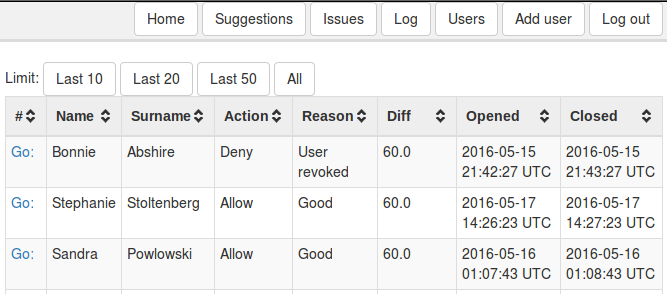
\includegraphics[width=1\textwidth]{PageLog.png}
	\caption{Mājaslapas žurnāla ekrānšāviņš izstrādes laikā}
	\label{fig:PageLog}
\end{figure}
Tā izskatās mājaslapas galvenā funkcija - žurnalēšana, šeit no administratora skata. Iespējams ierobežot redzamo žurnāla ierakstu skaitu. Parādīti lietotāju vārdi, uzvārdi, veiktā darbība (vai durvis tika atvērtas, vai nē), darbības iemesls, durvju atvēršanās un aizvēršanās laiki, \textit{diff} norāda atšķirību starp tiem. Sistēma izveidota tā, lai administrators redzētu visu lietotāju pieejas laikus, bet lietotāji spētu redzēt tikai savu pieejas vēsturi. Redzams, ka izmantotas \textit{Bootstrap} satvara \textit{CSS} klases pogām un tabulai. Bultiņas tabulas augšā norāda, ka ir iespējams kārtot tabulu, kas panākts ar \textit{tablesorter} spraudni.

\begin{figure}[H]%!ht
	\centering
	\captionsetup{justification=centering}
	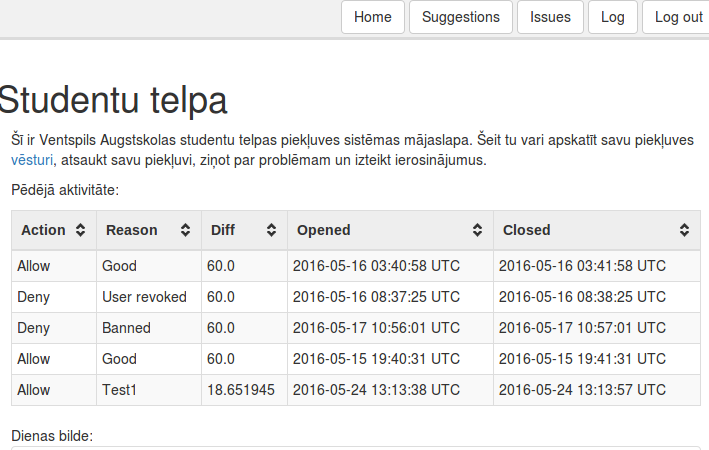
\includegraphics[width=1\textwidth]{PageUser.png}
	\caption{Mājaslapas lietotāja sākumlapas ekrānšāviņš izstrādes laikā}
	\label{fig:PageUser}
\end{figure}
Apmēram šādi izskatās mājaslapas sākumlapa no lietotāja skata punkta. Kā redzams, lietotājam ir dotas mazāk saites, nekā lapas administratoram, kā arī parādītais žurnāls attēlo tikai lietotāja pēdējo aktivitāti.
Kā viena no mazāk svarīgajām prasībām, kas padara mājaslapu jaukāku, ir dienas bildes iespēja (nav attēlota ekrānšāviņā), kura parādās sākumlapā.

\subsubsection{Bootstrap}
Darbā izmantots Bootstrap \textit{CSS}  satvars (\url{http://getbootstrap.com/}), kas ļauj ātri izveidot pieņemamas, arī mobilām iekārtām piemērotas mājaslapas.
Bootstrap ir iespējams pievienot \textit{Rails} aplikācijai vairākos veidos. Viens no veidiem ir pievienot to \textit{Gemfile}, kā bibliotēku. Tomēr tādu variantu neizvēlējos, jo tādejādi mājaslapas lietotājam būtu jālejuplādē Bootstrap \textit{CSS}  faili no uzstādītā servera, kā arī tas nav nepieciešams, ja negrasās ievērojami konfigurēt Bootstrap \textit{CSS}  klases.
Tā kā darbā nav paredzēts izmainīt Bootstrap klases, tas pievienots izmantojot satura piegādes tīklu (angl. \textit{content delivery network}) jeb \textit{CDN}, kas nodrošina augstu pieejamību \textit{CSS}  failiem. Kā arī, daudzas populāras mājaslapas izmanto Bootstrap, tādejādi ir iespējams, ka izveidotās mājaslapas lietotājiem, nepieciešamais \textit{CSS}  fails atrastos pārlūka kešatmiņā.
\begin{lstlisting}[language=HTML]
<link rel="stylesheet" href="https://maxcdn.bootstrapcdn.com/bootstrap/3.3.6/css/bootstrap.min.css" integrity="sha384-1q8mTJOASx8j1Au+a5WDVnPi2lkFfwwEAa8hDDdjZlpLegxhjVME1fgjWPGmkzs7" crossorigin="anonymous">
\end{lstlisting}

\subsubsection{\textit{jQuery}}
Mājaslapai ir nepieciešams \textit{jQuery} \textit{JavaScript}  satvars, lai nodrošinātu lietotāju žurnālu kārtošanu pēc datubāzes kolonnām. Izmantojot \textit{jQuery} \textit{tablesorter} spraudni (\url{https://mottie.github.io/tablesorter/docs/index.html}), tiek nodrošināta parādīto ierakstu kārtošana, atvieglojot sistēmas administrēšanu.

\subsection{Testēšana} \label{Testing}

\subsubsection{\textit{Codacy}}
\textit{Codacy} ir viens no statiskas koda analīzes servisiem, kas pieejams par brīvu atvērtā koda projektiem, kā arī ir viegli integrējams ar \textit{GitHub} (\url{https://github.com/integrations}). Statiska koda analīze spēj atklāt vairākas lietas neizpildot kodu.
Piemēram, iespējams atklāt:
\begin{itemize}
	\item koda stila kļūdas, kas parasti izveidojas nesekojot vispār pieņemtai konvencijai, tādejādi apgrūtinot koda lasāmību;
	\item neizmantotu kodu;
	\item drošības riskus, piemēram, \textit{SQL} injekcijas iespējas;
\end{itemize}
Statiska koda analīze spēj atklāt un izvairīties no zināmu sliktu paņēmienu izmantošanas, nodrošinot augstāku koda kvalitāti. Kvalitatīvs kods ir vieglāk lasāms un tādejādi arī vieglāk uzturams un atbalstāms.

\subsubsection{\textit{TravisCI} }
\textit{TravisCI}arī ir viens no CI rīkiem, kas ir viegli integrējams ar GitHub.
\begin{lstlisting}
	language: ruby
	rvm:
	  - 2.2.3
	bundler_args: --without production
	env:
	  - DB=sqlite
	script:
	  - RAILS_ENV=test bundle exec rake --trace db:migrate test
	  - bundle exec rspec
	notifications:
	  email: false
\end{lstlisting}
Izstrādes \textit{.travis.yml} fails \textit{TravisCI} konfigurēšanai. Šeit tiek norādīta uz kuras \textit{Ruby} valodas versijas ir jāveic testi un kura ir izvēlētā datubāze. Izstrādes laikā tika izmantota vienkāršā \textit{SQLite} datubāze. \textit{Script} blokā iespējams norādīt izpildāmās komandas. Ikreizi, kad tiks veiks iesūtījums uz \textit{GitHub}, \textit{TravisCI} veiks nepieciešamo \textit{Ruby} bibliotēku iegūšanu ar \textit{Bundler}, datubāzes migrēšanu, kā arī \textit{RSpec} testu izpildi.

\subsubsection{RSpec}
\textit{RSpec} ir populārākā \textit{Ruby} testēšanas bibliotēka. \textit{RSpec} ir BDD testēšanas satvars. \textit{RSpec} izmanto savu DSL, kas līdzinās dabiskas valodas specifikācijai. Lasot \textit{RSpec} testus tiem būtu jāizklausās pēc normāliem teikumiem. Tā \textit{RSpec} cenšas testus padarīt lasāmus un saprotamus. \cite{shayRspec}
\begin{lstlisting}
	describe "GET #index" do
    it "returns http success" do
      get :index
      expect(response).to have_http_status(:success)
    end
  end
\end{lstlisting}
Tipisks kontroliera tests.

\subsubsection{Shoulda matchers}
\textit{Shoulda matchers} ir \textit{RSpec} paplašinājums ar kuru iespējams vienkāršot daudzus testus un uzrakstīt tos vienā rindā.
\begin{lstlisting}
RSpec.describe User, type: :model do
	it { should have_many(:logs) }
	it { should have_secure_password }
	it { should validate_presence_of(:name) }
\end{lstlisting}
Šādi tiek pārbaudīts, vai lietotāja modelim ir pareizās asociācijas datubāzē, droši tiek saglabāta parole, izmantojot \textit{bcrypt} bibliotēku. Kā arī tiek apskatīts, vai \textit{Rails} pārliecinās, ka, pievienojot jaunu lietotāju, tiek ievadīts tā vārds.

\subsubsection{Faker}
\textit{Faker} ļauj uzģenerēt neīstus datus. Tas tika izmantots, lai piepildītu datubāzi ar vairākiem lietotājiem un piekļuves laikiem, lai veiktu aplikācijas demonstrācijas.
\begin{lstlisting}
	5.times do
	  User.create!(
	    name: Faker::Name.first_name,
	    surname: Faker::Name.last_name,
	    email: Faker::Internet.email,
	    card_id: Faker::Number.number(10),
	    level: 1,
	    password: 'password',
	    password_confirmation: 'password',
	    person_code: '123456-12340',
	    phone: Faker::PhoneNumber.cell_phone
	  )
	end
\end{lstlisting}
Izmantojot \textit{Ruby} \textit{.times} ciklu, šādi tika uzģenerēti neīsti sistēmas lietotāji.

\chapter{Secinājumi un ieteikumi}
Izstrādātā sistēma ir paredzēta tieši studentu darba telpas piekļuves pārvaldībai, tomēr tā ir pielāgojama jebkurai telpai, kurā piekļuves pārvaldība tiktu nodrošināta ar \textit{RFID} kartēm. Tā kā darba izstrādes gaitā nebija pieejams \textit{RFID} karšu lasītājs, tā darbība tika imitēta.
Izveidotā mājaslapa skaidri attēlo lietotāju telpas piekļuves mēģinājumu laikus
un sistēmas veikto darbību - durvu atvēršanu vai piekļuves liegšanu. Sistēma ļauj tās administratoram redzēt un pārvaldīt visu lietotāju piekļuvi, kā arī katram lietotājam ir iespējams redzēt savu piekļuves vēsturi. Lietotāji var arī izteikt ieteikumus un sūdzības.

Šajā darbā izveidoto pārvaldības mājaslapu ir paredzēts uzstādīt uz
\textit{RaspberryPi} vienplates datora un pie tā pievienot \textit{RFID}
karšu lasītāju un kameru. Visu izveidoto sistēmu paredzēts novietot studentu darba telpā.
Tomēr servera uzstādīšana ir veikta izmantojot infrastruktūra kā koda rīku \textit{Chef}, kas ļauj mājaslapu ātri un vienkārši uzstādīt uz jebkura servera vai virtuālās mašīnas. Šādā gadījumā jāparūpējas, ka karšu lasītājs sūta datus uz uzstādīto serveri.

Ieviešot šādu sistēmu, tiks būtiski palielināta drošība salīdzinot ar esošo sistēmu, jo jaunā sistēma nodrošina katra elektronikas studentu darba telpas piekļuves mēģinājuma žurnalēšanu. Sistēmai būtu arī jāpalielina elektronikas studentu apmierinātība ar darba telpu, jo piekļuve tai tiktu praktiski nodrošināta jebkurā diennakts laikā. Tiktu uzlabota telpas uzraudzība, kā arī jaunā sistēma ļautu izvairīties no sociālās inženierijas mēģinājumiem.

Veicot izmaiņas piekļuves iegūšanas procesā, to novirzot no iesnieguma iesniegšnas Augstskolas administrācijā uz tā iesniegšanu zinošam elektronikas darba telpas administratoram, kuram ir dotas sistēmas administrēšanas iespēja, varētu būtiski paātrināt piekļūšanu darba telpai. Noteiktajam darba telpas administratoram dodot iespēju izsniegt piekļuves \textit{RFID} kartes, piekļuves gaidīšanas periods varētu samazināties no vienas nedēļas, kā notiek pašreizējā sistēmā, uz piekļuves iegūšanu tajā pašā dienā. Kā arī darba telpas administratoram būtu iespēja liegt nekārtīga studenta piekļuvi telpai, ko pašreizējā sistēma īsti nepieļauj.

Darbs ir iesākts izmantojot labus paņēmienus. Pirmkārt, viss kods ir pieejams \textit{GitHub} servisā, otrkārt izmantotās integrācijas nodrošina pastāvīgu koda testēšanu:
\begin{describe}
	\item Mājaslapas izstrāde -- https://github.com/RihardsT/access_page
	\item Servera konfigurēšana -- https://github.com/RihardsT/access_page_cookbook
	\item Teorētiskais apraksts -- https://github.com/RihardsT/thesis
\end{describe}

Kaut gan izstrādātā pārvaldības mājaslapa spēj apmierināt minimālās tai izteiktās prasības, to vēl būtiski ir iespējams uzlabot. Jāveic ievērojams darbs, lai padarītu to draudzīgāku tās lietotājiem, veicot \textit{CSS} uzlabojumus. Lai nodrošinātu, ka netiekt ieviestas regresijas jāuzraksta visaptverošāki un pilnīgāki testi, gan mājaslapai, gan infrastruktūras kodam. Nākotnē varētu uzstādīt arī automātisku mājaslapas un servera atjaunināšanu, kad kods tiktu atjaunināts repozitorija pamatzarā, izmantojot \textit{TravisCI}.

Darbā izvirzītie mērķi un uzdevumi ir sasniegti. Administrēšanas mājaslapa ir izveidota un tā ir viegli uzstādāma uz servera. Sistēmu ieviešot jāparūpējas par \textit{SSL} sertifikātu iegūšanu un uzstādīšanu, \textit{RFID} karšu lasītāja savienošanu ar serveri, kā arī kameras uzstādīšana, lai varētu veikt momentuzņēmumus, durvju atvēršanās laikā.
Kopumā, darba autors uzskata, ka izstrādātā sistēma būtu pielietojama arī citu telpu piekļuves pārvaldībai, kā lēts un spējīgs risinājums.